\documentclass{sigchi}

% Use this command to override the default ACM copyright statement (e.g. for preprints). 
% Consult the conference website for the camera-ready copyright statement.
\toappear{}



% Arabic page numbers for submission. 
% Remove this line to eliminate page numbers for the camera ready copy
\pagenumbering{arabic}


% Load basic packages
\usepackage{balance}  % to better equalize the last page
\usepackage{graphics} % for EPS, load graphicx instead
\usepackage{times}    % comment if you want LaTeX's default font
\usepackage{url}      % llt: nicely formatted URLs

% llt: Define a global style for URLs, rather that the default one
\makeatletter
\def\url@leostyle{%
  \@ifundefined{selectfont}{\def\UrlFont{\sf}}{\def\UrlFont{\small\bf\ttfamily}}}
\makeatother
\urlstyle{leo}


% To make various LaTeX processors do the right thing with page size.
\def\pprw{8.5in}
\def\pprh{11in}
\special{papersize=\pprw,\pprh}
\setlength{\paperwidth}{\pprw}
\setlength{\paperheight}{\pprh}
\setlength{\pdfpagewidth}{\pprw}
\setlength{\pdfpageheight}{\pprh}

% Make sure hyperref comes last of your loaded packages, 
% to give it a fighting chance of not being over-written, 
% since its job is to redefine many LaTeX commands.
\usepackage[pdftex]{hyperref}
\hypersetup{
pdftitle={SIGCHI Conference Proceedings Format},
pdfauthor={LaTeX},
pdfkeywords={SIGCHI, proceedings, archival format},
bookmarksnumbered,
pdfstartview={FitH},
colorlinks,
citecolor=black,
filecolor=black,
linkcolor=black,
urlcolor=black,
breaklinks=true,
}

% create a shortcut to typeset table headings
\newcommand\tabhead[1]{\small\textbf{#1}}


% End of preamble. Here it comes the document.
\begin{document}

\title{Campus Sherpa}

\numberofauthors{4}
\author{
  \alignauthor Christopher Ford\\
    \email{cjford@mit.edu}\\
  \alignauthor Ganesh Ajjanagadde\\
    \email{gajjang@mit.edu}\\  
  \alignauthor Harihar Subramanyam\\
    \email{hsubrama@mit.edu}\\
   \alignauthor James Thomas\\
    \email{jjthomas@mit.edu}\\
}

\maketitle

\begin{abstract}
In this paper, we outline the motivation, development, and testing of Campus Sherpa, a mobile application for iOS 7 that allows users to make and take custom tours of the MIT campus. The app was inspired by a generative study which showed that people were unhappy with the one-size-fits-all approach of traditional campus tours and desired a tourism experience which catered to the varying interests of tourists. So, Campus Sherpa was developed to allow users to create tours and take tours. It servers as a platform for students to make tours to remember their experience at MIT, and for visitors to take a tour which caters to their interests at MIT. Our field evaluation, conducted after the development of our application, showed us that our Campus Sherpa was perfectly suited to improve upon the tour taking experience at MIT. (TODO: INCORPORATE FIELD STUDY RESULTS HERE)

\end{abstract}

\keywords{
	Geolocations; campus; tours; location tracking; tourism; campus; sharing
}
% Stubbed out these sections for now, don't know what to do with them

%\keywords{
%	Guides; instructions; author's kit; conference publications;
%	keywords should be separated by a semi-colon.
%	\textcolor{red}{Mandatory section to be included in your final version.}
%}
%
%\category{H.5.m.}{Information Interfaces and Presentation (e.g. HCI)}{Miscellaneous}
%
%See: \url{http://www.acm.org/about/class/1998/}
%for more information and the full list of ACM classifiers
%and descriptors. 
%\textcolor{red}{Mandatory section to be included in your
%final version. On the submission page only the classifiers'
%letter-number combination will need to be entered.}

\section{Introduction}

Every day, MIT receives a a large number of visitors from different backgrounds. The visitors include tourists exploring Boston/Cambridge, prospective undergrads, prospective grad students, middle/high schoolers attending Splash, researchers attending a conference, and professionals attending an event or career fair. Each visitor has different interests when visiting. For instance, an incoming freshman may be focused on exploring the undergraduate residence while a prospective biology graduate student may be more interested in the biological research labs. However, many of these visitors will take a campus tour which will take them to the main sights at MIT (ex. the Student Center, gymnasium, auditorium, main hallway, and architecturally impressive computer science laboratory). However, this ``one-size-fits-all'' nature of the tour fails to take into account the interests of each visitor and show them all the sights that they would enjoy seeing.

Campus Sherpa is a tourism app focused on MIT. Users can create tours, which are sequences of locations associated with media (ex. pictures, audio narration). Users can take tours, which takes them on a guided trip to interesting sites on the MIT campus and shows them relevant media for each site.

Primary research questions include: ``How can we fix this with an easy to use mobile application?", ``Is a mobile application the right way to solve this problem?", and ``How can we take advantage of modern cell phone technologies to make the use of our application as easy as possible?"

The goal of this application is to allow users to pursue a tour (likely after the main campus tour) which will help them make the most of their time at MIT. For instance, a prospective graduate student in Biology would follow a tour of the biology labs while a tourist interested in history would be taken to the most historically important sites at MIT. 

Since smartphones offer location awareness and mobility, they are the obvious platform choice for this application. By deploying this application for iOS, users can take out their smartphone when they arrive at MIT, select a tour based on their interest, and then begin exploring sites that will be most useful to them. 

The second aspect of this application is to allow users to chronicle their tours and share them with others. As prospective students compare MIT to other schools or as tourists reminisce about their visit to MIT, the ability to record their tours (by associating locations with text, photos, videos, and links to related content) will aid them in remembering. For current students, this offers a way to record the precious memories they make at MIT and share them with others.

Thus, the primary audience will be people who aim to tour MIT and record their experience there. The secondary audience will be current MIT students who would like to chronicle their lives at MIT. While some MIT tours will be pre-installed, the majority should be user-created. 

Based on our own experiences and the results of our interviews, people have varied tastes and desired destinations when visiting MIT, and we aim to make sure that their trip to MIT is as enjoyable and productive as possible. By creating an application to let users create, share, and follow custom tours of MIT, we hope to make college tours custom fit to each person�s taste, to make memories of MIT easy to record and share, and to make a platform for sharing tours.

\section{Related Works}

There exist a number of products and applications aimed at making tour taking more exciting and enjoyable. Interactive exhibits at museums and college campuses aim to improve upon the tour taking experience by allowing tour takers to interact with what they are touring. These interactive kiosks often serve many tourists at once, and fail to provide a custom tailored experience to each user. Often, these interactive stations can get bogged down with traffic, resulting in long wait times which only frustrates the tourist.

There exist a few mobile applications that try to enrich tourism as well. Applications in this domain fall into two main categories: applications that try to replace the tour taking experience all together, and applications that try to supplement existing tours. Applications in the first category include the Library of Congress Virtual Tour, Canadian Museum of Civilization, and American Museum of Natural History mobile applications. Although these virtual tours allow more users to "explore" a tourist destination, they fail to replicate the experience of touring in person. A 3.5" to 5" screen is not a good way to replicate a tour.

Applications that try to supplement existing tours include: the Boston Freedom Tail, Walking Cinema: Murder on Beacon Hill, and LAT Star Walk mobile applications. These applications do take in the users position so they can serve them content when they reach specific locations, but they lack the ability to create and share custom tours made by other users. With these applications, users are limited to the content made by the developers. While these applications usually only provide users with information specific to one tour, Campus Sherpa allows users to browse and take many tours of MIT, as created by other users.

TODO: ADD ACADEMIC RELATED WORKS

\section{Background}

Motivated by the above observation, we first identified the types of people touring MIT. We decided that for the purposes of campus tours, we can broadly classify people as current students, prospective freshmen, parents, and tourists. In order to gather information about these groups, we conducted a survey of these four groups, with some questions common to all four groups and some tailored to a specific group. We reached out to tour groups, classmates/colleagues, and friends/family. Each participant was interviewed for approximately 15 to 20 minutes. Here are some of the questions we asked:

\textbf{Everyone}:

\begin{itemize}
	\item What is the most memorable site you've visited here? Why?
	\item What is the one thing you most wish to see here? Why?
	\item Have you gone on a tour of MIT?
	\begin{enumerate}
		\item Are there any questions the tour guide didn't answer?
		\item Did the tour take you everywhere you wanted?
		\item Did the tour leave out any place you wanted to see?
	\end{enumerate}
\end{itemize}

\textbf{Current Students}:
\begin{itemize}
	\item What are three things you looked for when touring MIT?
	\item What is one place that the tour didn't cover, which you think tourists should see?
\end{itemize}

\textbf{Prospective Freshman}:
\begin{itemize}
	\item If you could ask a current student one question about MIT, what would it be?
	\item What aspect of MIT do you want explore the most?
\end{itemize}

\textbf{Parents}:
\begin{itemize}
	\item What are three places you want to tour at MIT that you think your child might not want to?
	\item If you could ask a current student one question about MIT, what would it be?
\end{itemize}

\textbf{Tourists}:
\begin{itemize}
	\item How long will you be visiting MIT?
	\item In a sentence, why did you want to come visit MIT?
\end{itemize}

Approximately twenty people responded to the survey, evenly distributed across the four demographics. Some of the responses to the survey are:

``There are always too many things to see \ldots I am wishing I can see more later'' (current student)

``Campus Preview Weekend (CPW) was really rushed, and I did not get to see everything'' (prospective freshman)

``I wish I could get a better sense of MIT culture. The tour guide briefly touched on how each dorm was different, but did not go into detail. '' (prospective freshman)

``I wish they had shown us where the students hang out '' (parent)

``I wish I could get a better sense of MIT culture. The tour guide briefly touched on how each dorm is different, but didn't go into detail. '' (tourist)

From the above responses, we saw that a common complaint was that people were not able to visit places they wanted to with the regular campus tours. In order to solve this problem, we proposed an application that helps create and share custom tours of the MIT campus called ``Campus Sherpa''.

Since smartphones offer location awareness and mobility, they are the obvious platform choice for ``Campus Sherpa''. By deploying this application for iOS, users can take out their smartphone when they arrive at MIT, select a tour based on their interest, and then begin exploring sites that will be most useful to them.

The second aspect of ``Campus Sherpa'' that we wished to support is to allow users to chronicle their tours and share them with others. As prospective students compare MIT to other schools or as tourists reminisce about their visit to MIT, the ability to record their tours (by associating locations with text, photos, videos, and links to related content) will aid them in remembering. For current students, this offers a way to record the precious memories they make at MIT and share them with others. Thus, the primary audience will be people who aim to tour MIT and record their experience there. The secondary audience will be current MIT students who would like to chronicle their lives at MIT.

While some MIT tours will be pre-installed, the majority should be user-created.
Based on our own experiences and the responses to our survey, people have varied tastes and desired destinations when visiting MIT, and we aimed to make sure that their trip to MIT is as enjoyable and productive as possible.

By creating an application to let users create, share, and follow custom tours of MIT, we hope to make college tours custom fit to each person's taste, to make memories of MIT easy to record and share, and to make a platform for sharing tours.

\section{System Description}

``Campus Sherpa'' allows users to achieve two goals: 

\begin{itemize}
	\item Take custom tours
	\item Create tours based on experiences.
\end{itemize}

When users launch the application, they are presented with a screen (Figure \ref{fig:Figure2}a) that lists all tours that have been created (by any user). If they would like to take a tour, they can select one from the list, and they will be directed to a "Start Tour" page (Figure \ref{fig:Figure2}b), which includes a map of all of the locations on the tour. If any of the location pins are clicked, the name of the corresponding location is shown.

Once the user starts a tour, they are presented with a screen for the first location. The screen contains a picture of the location, two buttons for navigating to the previous location and the next location, another button that brings up a map with all of the locations (the same map from Figure \ref{fig:Figure2}b), and a final button that shows a list of media items associated with the current location (Figure \ref{fig:Figure2}c).

\begin{figure}
\centering
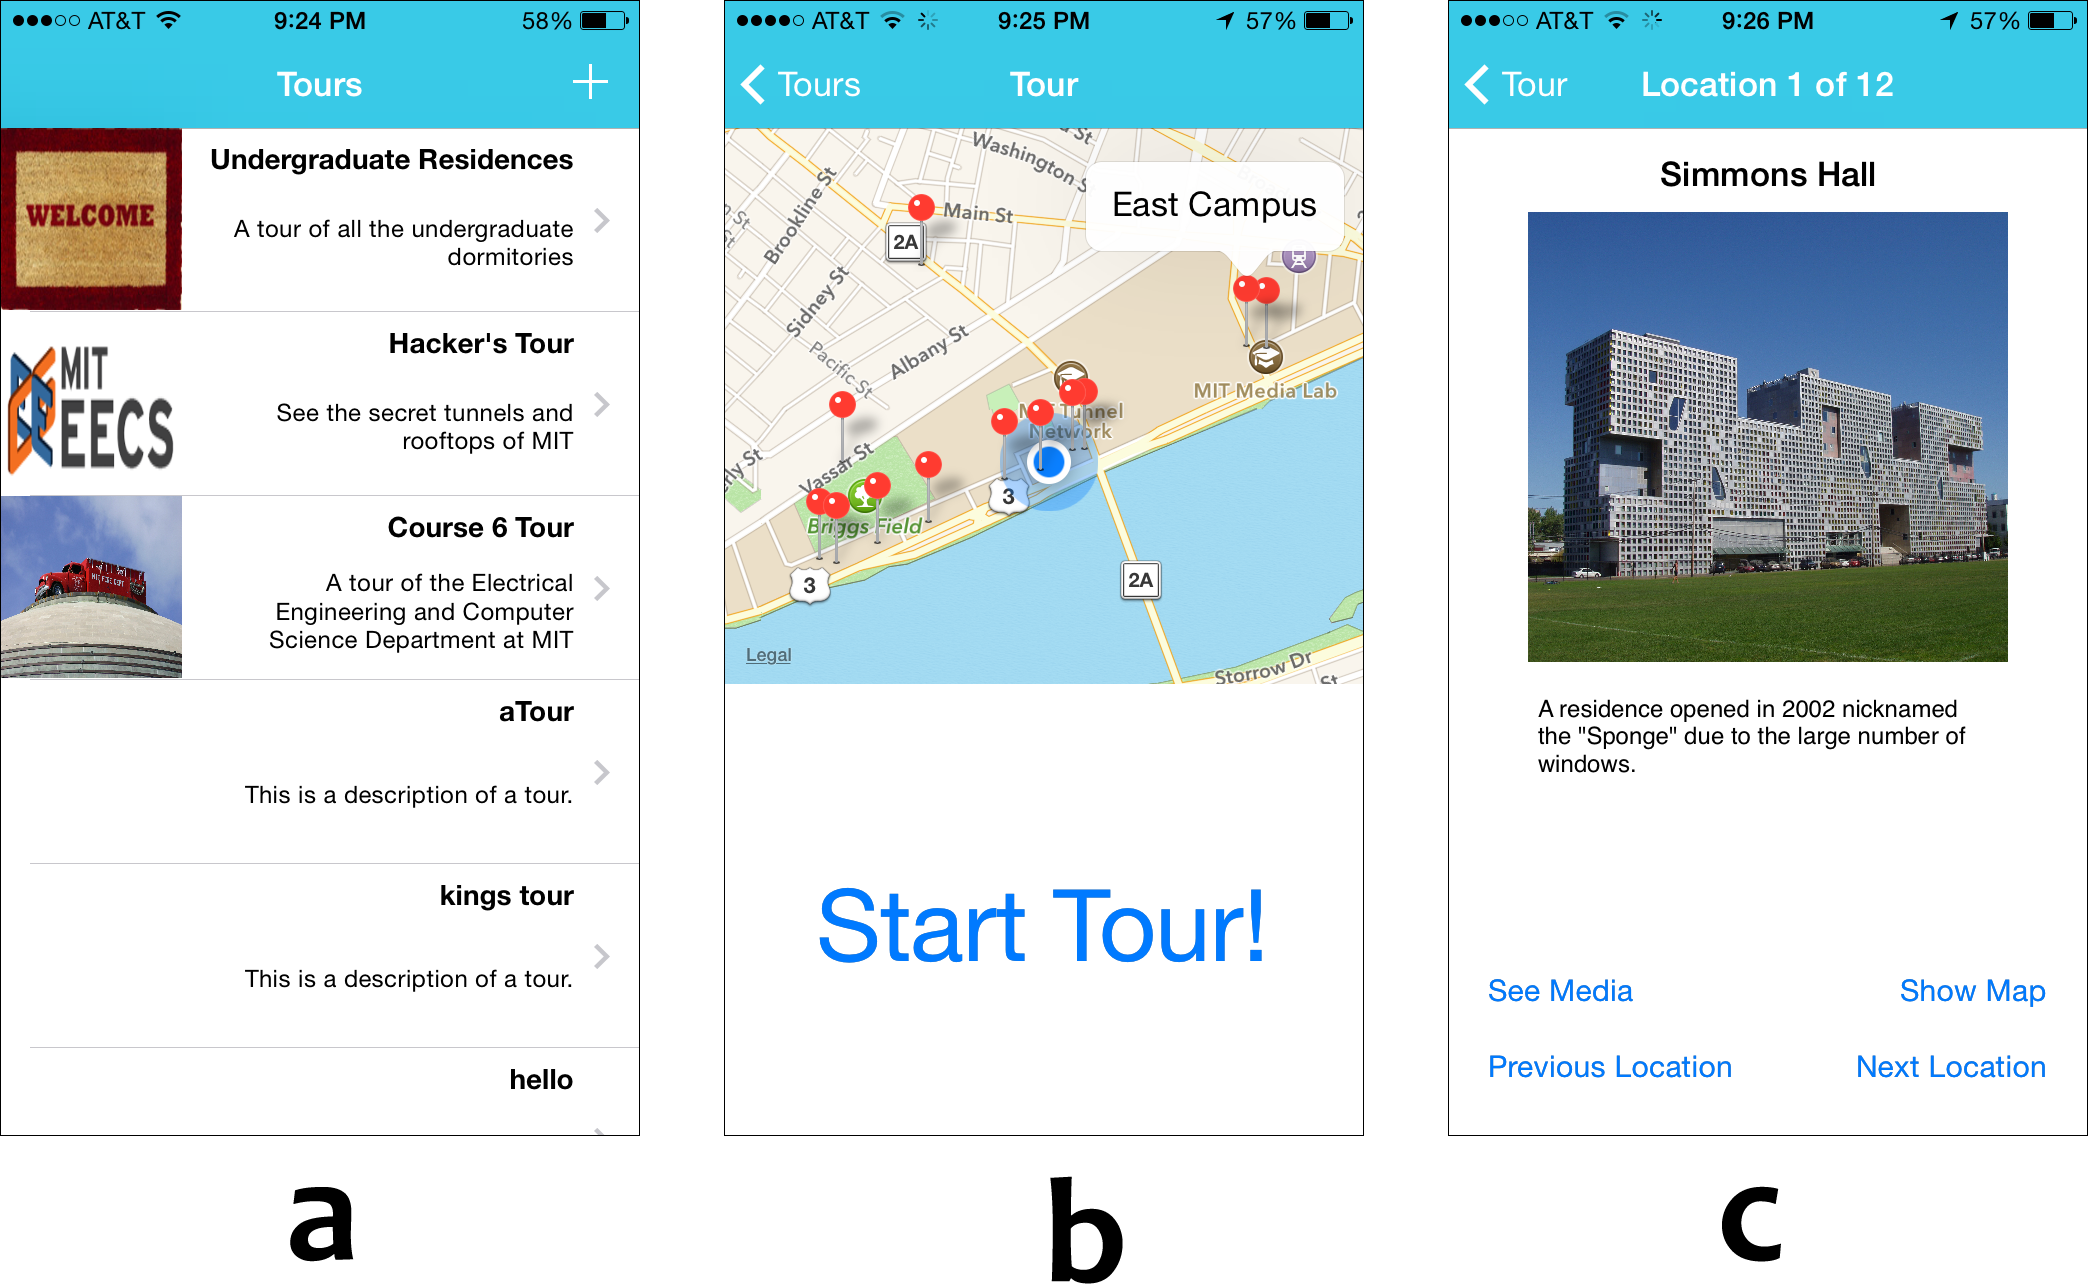
\includegraphics[width=1.0\linewidth]{./Figure2}
\caption{The screens of Campus Sherpa. (a) shows the tour browsing screen, where users can search for tours. (b) shows the tour preview screen, where users can preview the locations on the tour. (c) shows the location screen, where users can read about a locations and access associated media.}
\label{fig:Figure2}
\end{figure}


\subsection{Technical Details}
We use Parse for the backend. Parse is a backend-as-a-service which provides an SDK for iOS which allows users to persist objects on the server. This is much simpler than building a backend from scratch. For this project, we persist and retrieve latitude/longitude, text, pictures, and audio - which Parse supports. Since this application does not run in a browser, we do not have any browser dependencies (TODO: EXPAND THIS)
    
\section{Field Study}

<<<<<<< HEAD
For our field study, we decided to combine quantitative and qualitative analysis of Campus Sherpa's user experience. For each user, we tracked which screens were viewed most often, which buttons were pressed most frequently, and for how much time a particular screen was viewed for. This gave us a sense of what our users were interacting with, or getting stuck on, from a quantitative perspective.

We also kept a detailed log of how we observed our users interacting with Campus Sherpa. We observed and noted body language and facial expression and did our best to map both positive and negative interactions with our application to specific screens.

Additionally, we surveyed users after they tried our application to get some of their feedback as well. User feedback, combined with qualitative observations, and quantitative data gave us a detailed look into how well Campus Sherpa worked for our users.


Since our app is targeted at tourists of MIT, a demographic we did not have ready access to, we primarily focused on gathering information from two more available groups: iOS experts, who could critique the user experience of the app, and recent prefrosh (current MIT freshmen), who could asses the app's utility for prospective students. We had 4 students from each group take one tour (a brief tour of some locations in the Infinite Corridor) and make one tour, and we took notes on any difficulties they seemed to be experiencing while using the app. After they finished both tasks, we asked them for any feedback they had. We used a few standard questions:
\begin{itemize}
\item What additional features might it be useful for this app to have?
\item Was any part of the user experience awkward or difficult?
\item Do you see this app being useful in its current form to prospective tourists? What advantages would it have over tour guide-led tours?
\end{itemize}
We received a large volume of feedback. Some of the most common responses and insights follow:
\begin{itemize}
\item The "Show Map" screen (visible when taking a tour, looks much like Figure \ref{start-tour}) should have shown the pin for the current location in a different color.
\item The keyboard on many screens was hard to dismiss -- the iOS experts suggested converting many of the views to ScrollViews so that users could scroll down to see elements obscured by a keyboard.
\item If one location has a picture and the subsequent location does not (when taking a tour), the subsequent location's picture is set to the first location's picture, causing confusion.
\item The workflow for the make tour portion of the app was a bit confusing -- the "Publish Tour" button appeared too early, so users sometimes clicked it before adding any locations to the tour.
\item It would be nice if the app provided users directions to get one from one location to the next.
\end{itemize}
We modified the app to address the most common concerns of the testers. An interesting use case we discovered from running the field study is that many users actually like to step through tours in the app without actually moving physically from place to place. Thus, our app could prove incredibly useful to prospective students who are unable to visit the campus but want a sense for the rich variety of locations and sights at MIT. This use case could also help people plan what places they would like to visit during a trip to MIT. In essence, the app, if populated with a sufficient number of user-generated tours, could serve as a catalog of all of the interesting sets of related locations on campus.
>>>>>>> Some work on the field study portion

After they tested the app, the testers were asked to fill out a brief survey consisting of the following questions, with responses being ratings on a 1-to-5 scale:
\begin{itemize}
\item How useful do you think this app would have been for you during CPW?, with 1 being "Don't think tours would have played a big role in my decision, or tour guide-led tours would have been more than enough" and 5 being "Seeing different parts of campus would have been crucial to my decision, and this app would have helped me with that"
\item As a current MIT student, could you see yourself using this app to explore different parts of campus when you had some free time?, with 1 being "Not at all" and 5 being "Definitely"
\item Could you see this app being useful to tourists who want to get a better sense of MIT?, with 1 being "No, there are much better ways to do this" and 5 being "Yes, this app could offer much more information than tour guide-led tours or other options"
\end{itemize}
With the second question we explored yet another use case -- the physical tour for people who are already familiar with MIT in general but might want to explore a very niche part of campus. For example, there could be a tour with destinations popular for "hacking," which might include the roofs of various buildings and instructions on how to reach them. The results of this survey are plotted in Figure \ref{survey-results}.

\section{Discussion}

TODO: Add Discussion

\subsection{Future Work}

The next major milestone for Campus Sherpa is to create a recommendation system which suggests tours (or perhaps combine existing tours) that cater to a user's unique interests. This was omitted from this version of Campus Sherpa because 1) There weren't enough tours such that a recommendation system would be useful, and 2) The algorithmic and machine learning challenges of building a recommendation system were outside the scope of the class. Other improvements to the app include video support, tour ratings, and user profiles.

\subsection{Conclusion}

TODO: ADD CONCLUSION

\section{Acknowledgments}

We thank the participants of our studies and exercises for their time and effort, as well as for allowing us
to use their thoughts and comments in both this paper, and in the development process of Campus Sherpa.

We also thank Ed Barrett, Frank Bentley, and Jason Martin Lipshin and the entire 21W.789 staff for their continued support and advice. Without them, Campus Sherpa would not have been possible.

% Balancing columns in a ref list is a bit of a pain because you
% either use a hack like flushend or balance, or manually insert
% a column break.  http://www.tex.ac.uk/cgi-bin/texfaq2html?label=balance
% multicols doesn't work because we're already in two-column mode,
% and flushend isn't awesome, so I choose balance.  See this
% for more info: http://cs.brown.edu/system/software/latex/doc/balance.pdf
%
% Note that in a perfect world balance wants to be in the first
% column of the last page.
%
% If balance doesn't work for you, you can remove that and
% hard-code a column break into the bbl file right before you
% submit:
%
% http://stackoverflow.com/questions/2149854/how-to-manually-equalize-columns-
% in-an-ieee-paper-if-using-bibtex
%
% Or, just remove \balance and give up on balancing the last page.
%
\balance

\section{References}

\bibliographystyle{acm-sigchi}
\bibliography{testbib}
\end{document}
